\documentclass{article}

\usepackage{fancyhdr}
\usepackage{extramarks}
\usepackage{amsmath}
\usepackage{amsthm}
\usepackage{amsfonts}
\usepackage{tikz}
\usepackage[plain]{algorithm}
\usepackage{algpseudocode}

\usetikzlibrary{automata,positioning}

%
% Basic Document Settings
%

\topmargin=-0.45in
\evensidemargin=0in
\oddsidemargin=0in
\textwidth=6.5in
\textheight=9.0in
\headsep=0.25in

\linespread{1.1}

\pagestyle{fancy}
\lhead{\hmwkAuthorName}
\chead{\hmwkClass\ (\hmwkClassInstructor\ \hmwkClassTime): \hmwkTitle}
\rhead{\firstxmark}
\lfoot{\lastxmark}
\cfoot{\thepage}

\renewcommand\headrulewidth{0.4pt}
\renewcommand\footrulewidth{0.4pt}

\setlength\parindent{0pt}

%
% Create Problem Sections
%

\newcommand{\enterProblemHeader}[1]{
    \nobreak\extramarks{}{Problem \arabic{#1} continued on next page\ldots}\nobreak{}
    \nobreak\extramarks{Problem \arabic{#1} (continued)}{Problem \arabic{#1} continued on next page\ldots}\nobreak{}
}

\newcommand{\exitProblemHeader}[1]{
    \nobreak\extramarks{Problem \arabic{#1} (continued)}{Problem \arabic{#1} continued on next page\ldots}\nobreak{}
    \stepcounter{#1}
    \nobreak\extramarks{Problem \arabic{#1}}{}\nobreak{}
}

\setcounter{secnumdepth}{0}
\newcounter{partCounter}
\newcounter{homeworkProblemCounter}
\setcounter{homeworkProblemCounter}{1}
\nobreak\extramarks{Problem \arabic{homeworkProblemCounter}}{}\nobreak{}

%
% Homework Problem Environment
%
% This environment takes an optional argument. When given, it will adjust the
% problem counter. This is useful for when the problems given for your
% assignment aren't sequential. See the last 3 problems of this template for an
% example.
%
\newenvironment{homeworkProblem}[1][-1]{
    \ifnum#1>0
        \setcounter{homeworkProblemCounter}{#1}
    \fi
    \section{Problem \arabic{homeworkProblemCounter}}
    \setcounter{partCounter}{1}
    \enterProblemHeader{homeworkProblemCounter}
}{
    \exitProblemHeader{homeworkProblemCounter}
}

%
% Homework Details
%   - Title
%   - Due date
%   - Class
%   - Section/Time
%   - Instructor
%   - Author
%

\newcommand{\hmwkTitle}{Homework 4.2}
\newcommand{\hmwkDueDate}{April 1, 2020}
\newcommand{\hmwkClass}{Engr 216}
\newcommand{\hmwkClassTime}{Section 509}
\newcommand{\hmwkClassInstructor}{Dr. O}
\newcommand{\hmwkAuthorName}{\textbf{Amari West}}
\newcommand{\hmwkDueTime}{11:55pm \\ 9 Pages}

%
% Title Page
%

\title{
    \vspace{2in}
    \textmd{\textbf{\hmwkClass:\ \hmwkTitle}}\\
    \normalsize\vspace{0.1in}\small{Due\ on\ \hmwkDueDate\ at \hmwkDueTime}\\
    \vspace{0.1in}\large{\textit{\hmwkClassInstructor\ \hmwkClassTime}}
    \vspace{3in}
}

\author{\hmwkAuthorName}
\date{}

\renewcommand{\part}[1]{\textbf{\large Part \Alph{partCounter}}\stepcounter{partCounter}\\}

%
% Various Helper Commands
%

% Useful for algorithms
\newcommand{\alg}[1]{\textsc{\bfseries \footnotesize #1}}

% For derivatives
\newcommand{\deriv}[1]{\frac{\mathrm{d}}{\mathrm{d}x} (#1)}

% For partial derivatives
\newcommand{\pderiv}[2]{\frac{\partial}{\partial #1} (#2)}

% Integral dx
\newcommand{\dx}{\mathrm{d}x}

% Alias for the Solution section header
\newcommand{\solution}{\textbf{\large Solution}}

% Probability commands: Expectation, Variance, Covariance, Bias
\newcommand{\E}{\mathrm{E}}
\newcommand{\Var}{\mathrm{Var}}
\newcommand{\Cov}{\mathrm{Cov}}
\newcommand{\Bias}{\mathrm{Bias}}

% Allow double underline
\def\doubleunderline#1{\underline{\underline{#1}}}

% Allow for units in math mode
\newcommand{\unit}[1]{\ensuremath{\, \mathrm{#1}}}

\begin{document}

\maketitle

\pagebreak

\begin{homeworkProblem}
	A weightless rectangular bar BDC is loaded as shown below. There is a smooth pin at point C, a 100 N force at point D and a cable at point B. The bar and all forces are in the plane of the page (2D Case).
	\\
	
	a) Write the 100 N force using polar vector representation: $F = |F| N$ @ angle $\theta$ CCW from +x to the right. Calculate the angle theta in degrees. Hint: see example in Lecture 8 (slide 19)
	\\
	
	b) Calculate the moment of the 100 N force about point C. Give your answer in N$\cdot$m (newton-meter).
	\\
	
	c) What should the direction of the 100 N force be to produce a zero moment about point A? Calculate and report the smallest angle in degrees CCW from +x to the right (angle in standard position)
	\\
	
	\begin{center}
		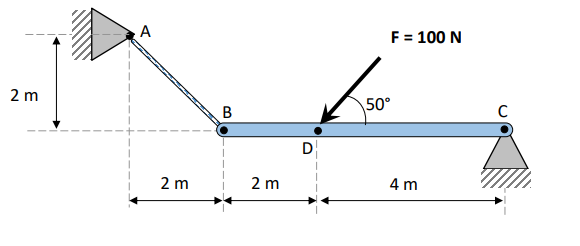
\includegraphics[scale=0.9]{problem1.png}
	\end{center}
	
	\textbf{Solutions:}
	\\
	
	a) 100 @ $230^{\circ}$ CCW
	\\
	
	b) 306.4 N$\cdot$m CW
	\\
	
	c) $\theta = 206.6^{\circ}$
	\\ 
		
\end{homeworkProblem}

\pagebreak

\begin{homeworkProblem}
	An asymmetric V-shaped bar ABC is attached to a surface at point A as shown below. The sides of the bar have the following lengths: AB = 160 mm, and BC = 200 mm. A force \textbf{F} = 500 N is applied at point C. The force vector is perpendicular to the side BC and points in the 4th quadrant assuming the standard orientation of the Cartesian xy-plane (with positive x-axis pointing right and positive y-axis pointing up).
	\\
	
	The bar and all forces are in the plane of the page (2D case).
	\\
	
	a) Calculate the moment of the force \textbf{F} about point A.
	\\
	
	b) Calculate the moment of the force \textbf{F} about point B.
	\\
	
	\textbf{Attention}: Convert millimeters to meters to give your answers in newton-meters, N$\cdot$m.
	\\
	
	\begin{center}
		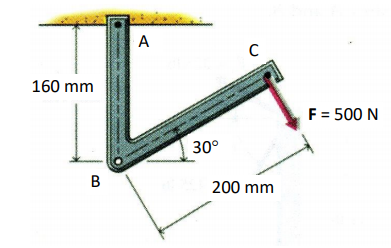
\includegraphics[scale=0.9]{problem2.png}
	\end{center}
	
	\textbf{Solutions:}
	\\
	
	a) $M_A$ = 60 N$\cdot$m CW
	\\
	
	b) $M_B$ = 100 N$\cdot$m CCW
	\\

\end{homeworkProblem}

\pagebreak

\begin{homeworkProblem}
	A uniform in shape and mass bar AB is supported by a smooth pin at point A. The orientation of the bar is given by angle theta, $\theta$, as shown below. An external force P is applied to the bar at point B. The direction of the force is given by angle phi, $\phi$, as shown below. Both angles theta and phi are angles in standard position. Not that $0 \leq \theta \le 2\pi$ and $0 \leq \phi \le 2\pi$. The weight of the bar is W; the length of the bar is L. The bar and all forces are in the plane of the page (2D case). The length is in meters and the forces are in newtons.
	\\
	
	Draw a free-body diagram for the bar AB; use the standard orientation of the Cartesian xy-plane (with positive x-axis pointing right and positive y-axis pointing up). Derive an expression for the net moment about point A in terms of given parameters like W, P, L, $\theta$, and/or $\phi$.
	\\
	
	\underline{\textbf{Given}}
	\\
	
	\begin{itemize}
		\item Known angle, $\theta$
		\item Known angle, $\phi$
		\item Known force, $\vec{P}$
		\item Known weight, $W$
		\item Known length, $L$
		\item Known points, A and B
	\end{itemize}
	
	\underline{\textbf{Find}}
		\begin{itemize}
			\item An equation for the net moment about point A.
		\end{itemize}
	
	\underline{\textbf{Diagram}}
	
	\begin{center}
	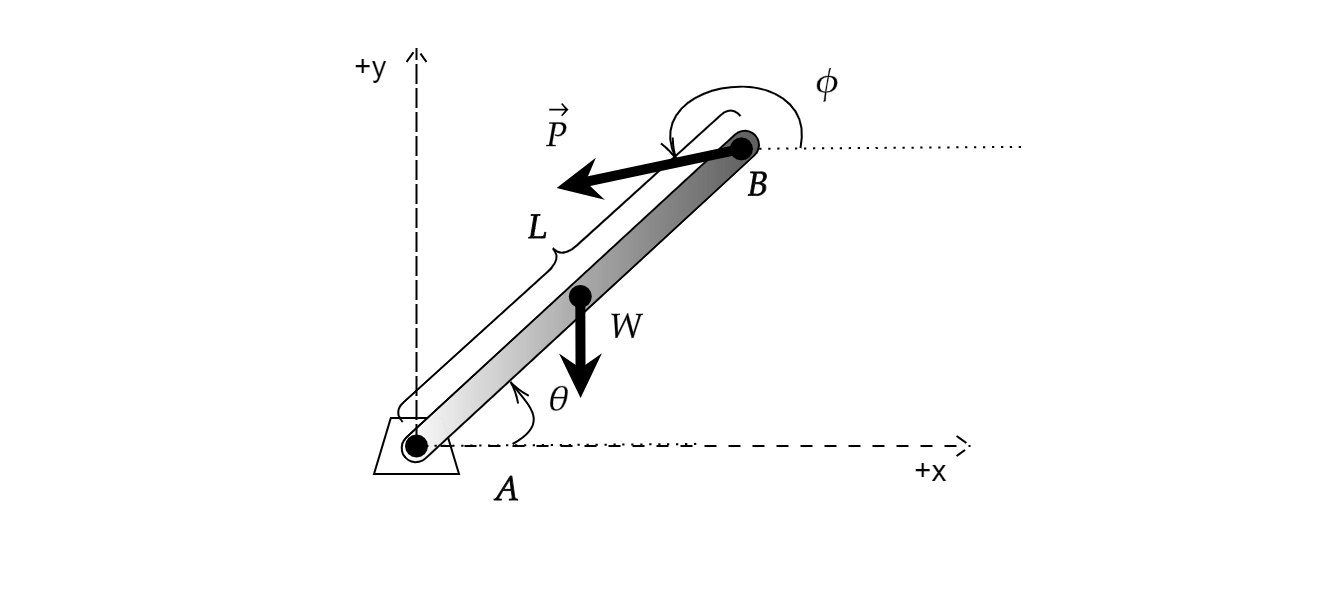
\includegraphics[scale=0.3]{problem3.png}
	\end{center}
	
	\underline{\textbf{Theory}}
	\\
	
	The moment of the force is found with the following equation:
	\[
	\begin{split}
		\vec{M} &= \vec{r} \times \vec{F}
		\\
		& = (r_xF_y - r_yF_x)\vec{k}
	\end{split}
	\]
	
	Essentially, deriving the moment involves the cross product of the force and distance vectors.
	
	\underline{\textbf{Assumption}}
	\\
	
	a) There is no friction in the model
	\\

	b) Point A is the pivot
	\\
	
	\underline{\textbf{Solution}}
	\\
	
	First, split all of the force and distance vectors into their components.
	
	\[
	\begin{split}
		\vec{P} &= |P|\cos(\phi)\hat{i} + |P|\sin(\phi)\hat{j}
		\\
		\vec{r}_P &= L\cos(\theta)\hat{i} + L\sin(\theta)\hat{j}
	\end{split}
	\]
	
	and
	
	\[
	\begin{split}
	\vec{W} &= |W|\cos(270^{\circ})\hat{i} + |W|\sin(270^{\circ})\hat{j}
	\\
	\vec{r}_W &= \frac{L}{2}\cos(\theta)\hat{i} + \frac{L}{2}\sin(\theta)\hat{j}
	\end{split}
	\]
	
	Now find the cross products of both vector pairs. 
	
	\[
	\begin{split}
	\vec{M}_P &= \begin{vmatrix}i & j & k \\ |P|\cos(\phi) & |P|\sin(\phi) & 0 \\ L\cos(\theta) & L\sin(\theta) & 0\end{vmatrix}
	\\
	&= (|P|\cos(\phi))(L\sin(\theta)) - (|P|\sin(\phi))(L\cos(\theta))
	\\
	&= |P|\cdot L (\sin(\theta - \phi)) 
	\end{split}
	\]
	
	and
	
	\[
	\begin{split}
	\vec{M}_P &= \begin{vmatrix}i & j & k \\ |W|\cos(270^{\circ}) & |W|\sin(270^{\circ}) & 0 \\ \frac{L}{2}\cos(\theta) & \frac{L}{2}\sin(\theta) & 0\end{vmatrix}
	\\
	&= (|W|\cos(270^{\circ}))\frac{L}{2}\sin(\theta) - |W|\sin(270^{\circ})(\frac{L}{2}\cos(\theta))
	\\
	&= |W|\frac{L}{2}(\sin(\theta - 270^{\circ}))
	\end{split}
	\]
	
	The equation for the net moment is
	
	\[
	\vec{M}_{net} = |P|\cdot L (\sin(\theta - \phi)) + |W| \frac{L}{2}(\sin(\theta - 270^{\circ}))
	\]
	
	\underline{\textbf{Conclusion}}
	\\
	
	After solving for the cross product of both forces and their relative distance to point A, the final equation derived was
	
	\[
	\vec{M}_{net} = |P|\cdot L (\sin(\theta - \phi)) + |W| \frac{L}{2}(\sin(\theta - 270^{\circ}))
	\]
	
\end{homeworkProblem}

\pagebreak

\begin{homeworkProblem}
	Two large balls roll over a smooth surface and collide. They are made of a super hard material so there is no deformation. Ball 1 has a mass $m_1$ of 2.00 kg and travels with an initial velocity 10.0 m/s at $0^{\circ}$ CCW. Ball 2 has a mass $m_2$ of 5.00 kg and travels with an initial velocity of 1.42 m/s at $60^{\circ}$ CCW. After the collision the direction of the velocity vector of ball 1 is $20^{\circ}$ CCW and the direction of the velocity vector of ball 2 is $350^{\circ}$ CCW.
	\\
	
	a) Calculate the velocity of ball 1 after the collision.
	\\
	
	b) Calculate the velocity of ball 2 after the collision.
	\\
	
	\textbf{Solutions:}
	\\
	
	a) $v_1 = 10.14$ m/s
	\\
	
	b) $v_2 = 0.9106$ m/s
	\\
	
\end{homeworkProblem}

\pagebreak

\begin{homeworkProblem}
	A villain with mass 70.0 kg runs at a velocity of 10.0 m/s at $180.0^{\circ}$ CCW into Chuck Norris' fist moving at a speed of 0.100 m/s at $0.0^{\circ}$ CCW. The villain is knocked back and is now moving at a velocity of 9.44 m/s at $20.0^{\circ}$ CCW, and Chuck Norri' fist moves at a velocity of 0.0500 m/s at $350^{\circ}$.
	\\
	
	a) Draw a collision diagram similar to the diagram given in Problem 4
	\\
	
	b) What is the mass of Chuck Norris' fist in kg?
	\\
	
	c) How much kinetic energy is lost in the collision?
	\\
	
	\underline{\textbf{Given}}
	\\
	
	\begin{itemize}
		\item $v_{v1} = 10.0$ m/s @ $180.0^{\circ}$
		\item $v_{c1} = 0.100$ m/s @ $0.0^{\circ}$
		\item $v_{v2} = 9.44$ m/s @ $20.0^{\circ}$
		\item $v_{c2} = 0.0500$ m/s @ $350.0^{\circ}$
		\item $m_v = 70.0$ kg		
	\end{itemize}
	
	\underline{\textbf{Find}}
	\\
	
	b) The mass of Chuck Norris' fist in kg?
	\\
	
	c) The amount of kinetic energy lost in the collision
	\\
		
	\underline{\textbf{Diagram}}
	\\
	
	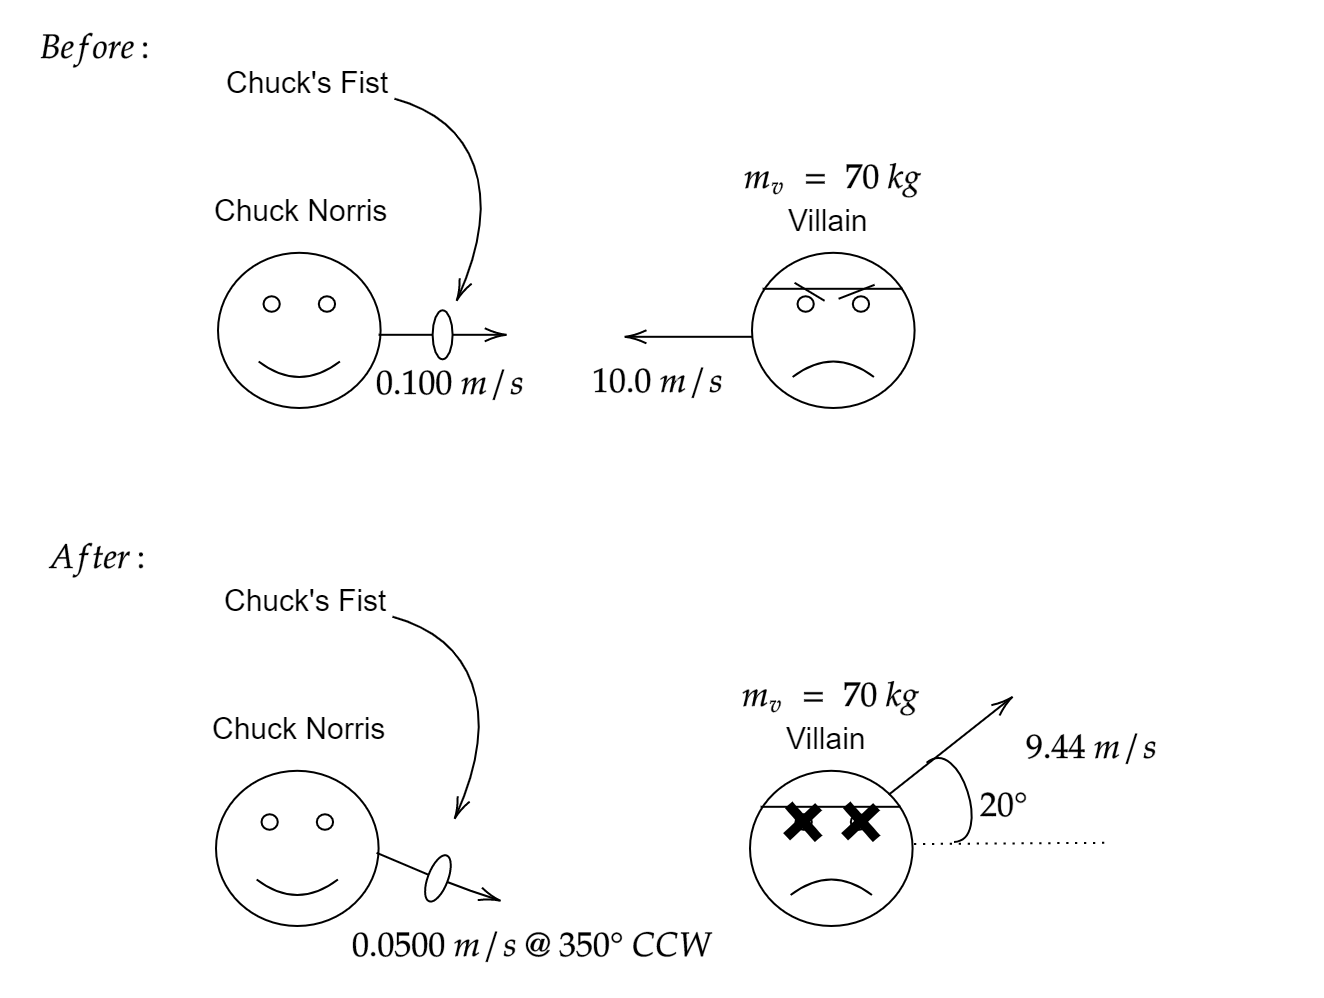
\includegraphics[scale=0.2]{problem5.png}
	
	\underline{\textbf{Theory}}
	\\
	
	This problem involves the conservation of momentum which means that the total momentum of the objects should not change before or after the collision as demonstrated mathematically below:
	
	\[
	\begin{split}
		\vec{P} &= m\vec{v}
		\\
		\vec{P}_{Before} &= \vec{P}_{After}
	\end{split}
	\]
	
	\underline{\textbf{Assumption}}
	\\
	
	a) This is an elastic collision.
	\\
	
	\underline{\textbf{Solution}}
	\\
	
	To find the mass of Chuck Norris' fist, set the momentum before equal to the momentum after and solve for the missing mass, $m_f$.
	
	\[
	\begin{split}
	70(10\cos(180^{\circ})) + m_f (0.100\cos{0^{\circ}}) &= 70(9.44\cos{20^{\circ}}) + m_f (0.05\cos(350^{\circ}))
	\\
	m_f &= 26018
	\end{split}
	\]
	
	To find any lost kinetic energy, subtract the initial kinetic energy from the final kinetic energy.
	
	\[
	\begin{split}
		\Delta KE &= KE_f - KE_i
		\\
		&= \frac{1}{2} m_i v_i^2 - \frac{1}{2} m_f v_f^2
		\\
		&= \frac{1}{2}\left[ 26018 ((0.1)^2 - (0.05)^2) + 70(10^2 - 9.44^2)\right] 
		\\
		&= \doubleunderline{481.7}
	\end{split}
	\]
	
	\underline{\textbf{Conclusion}}
	\\
	
	a) See Diagram Section
	\\
	
	b) $m_f = 26018$ kg
	\\
	
	c) $\Delta KE = 481.7$ 
\end{homeworkProblem}

\pagebreak

\begin{homeworkProblem}
	Ender and Shen are flying at each other during a battle in space. Ender moves with a velocity $v_1$ of 12 m/s at $30^{\circ}$ CCW and Shen, with a mass of 45 kg, moves at a velocity $v_2$ of 9.0 m/s at $135^{\circ}$ CCW. When the two collide, they hold on to each other and move with a velocity $v_3$ of 6.4 m/s at $75^{\circ}$ CCW. What is Ender's mass in kg?
	\\
	
	\textbf{Solutions:}
	\\
	
	a) $m_E$ = 41.21 kg
	
\end{homeworkProblem}

\end{document}
